\documentclass[a4paper]{article}
\usepackage{amsmath}
\usepackage{graphicx}
\usepackage{longtable}
\usepackage{makecell}
\usepackage[most]{tcolorbox}
\usepackage{listings}
\usepackage{csquotes}

\title{SDCND Behavioral Cloning}
\date{2019-04-22}
\author{Matthias Schinacher matthias.schinacher@googlemail.com}

\begin{document}

\maketitle
\tableofcontents
\newpage

\section{Intro}
The project is a homework assignment for Udacity's \textbf{Self Driving Car Nano Degree}.
The project is the 4th one called \textit{Behavioral Cloning}.
\\
The task is to train a neural network to mimic the driving recorded
by driving through a car- track simulation.
The goal accuracy is to be able to drive a whole lap within the simulation
\enquote{autonomously}, meaning by letting the (convolutional) neural network
do the driving (the NN actually only controls the steering angle, not all possible
input parameters).

\section{The project}
\subsection{Result files}
The project contains 2 sets of results, both of which actually manage to
do the autonomously lap. There are 2 slightly different models, the actual
training and validation data used was the same (a dataset named \enquote{test04}).

\begin{tabular}{ |l|l|l| }
  \hline
  model-file & model-program & video \\
  \hline
  \texttt{test04.cnn.model} & \texttt{model.py} & \texttt{model\_test04.mp4} \\
  \texttt{test04.cnn.model2} & \texttt{model2.py} & \texttt{model2\_test04.mp4} \\
  \hline
\end{tabular}

The second model is way bigger and github would not let me upload it, so I did split
the actual model file which could be reconstructed with:\\
\enquote{\texttt{cat test04.cnn.model2?? > test04.cnn.model2}}
\\
I copied the model-file and video of the 1st model to \enquote{model.h5} and
\enquote{video.mp4} as these were the defined expected file names.

\subsection{Implementation and experimentation}
I choose to implement everything on my local computer.

\paragraph{Step 1, acquiring training/validation data}
this was done locally several times by driving a few laps in the sim and
renaming the resulting simulation-log file.

\paragraph{Step 2, preprocessing}
I first wrote a preprocessing script (\texttt{preprocess.py}) that would gather
data from selected simulation runs (by taking the respective file names as input)
under a specified \enquote{training-set-name} and generate randomly shuffled
training/validation/test subsets thereof (70/20/10 %%).

\paragraph{Step 3, regression}
I then wrote a script (\texttt{simple\_regression.py}) that would try to learn a
simple regression model from the training data, that I could run with the simulation.\\
I hoped to get a better \enquote{feel} for the setup with this. But the my regression models
would not work as hoped in the simulation (the car kept driving of the track) and I
abandoned the regression model.

\paragraph{Step 4, the CNN models}
I then implemented a CNN model heavily inspired by the network I implemented for
the traffic signs. I did change some of the parameters. I first tried to use
a NN without dropout, but that would heavily overfit so I (re-) inserted drop-out layers.
\\
I also used the recommended flip- the image approach to get double the input data
and transformed the images to RGB colour space (as used by \enquote{drive.py}).
Both model implementations use the adam- optimizer to do the training for
simplification reasons.

\paragraph{Step 5, more training data}
At first I had difficulties with getting to the full lap (the car drove
into the water after half of it). I decided to heed the suggestion and collected
more training data by doing a training simulation where I explicitly drove towards
the sides of the track almost leaving it before I corrected the steering,
hoping the NN would learn to \enquote{drive back to the middle of the track}
by example.\\
\textbf{This seemed to have worked!} as the resulting model would achieve
the desired lap after using the new data \textit{in addition} to the previously used data.

\paragraph{1st CNN model version}
:\\
The python source \texttt{model.py} contains the first successful version of
the model I implemented, meaning the first version while playing with the
models layers (size, number, types of layers and their respective parameters),
that I could use to save a model that could steer the demanded full lap in
autonomous mode.
\\

Basic model features:
\begin{itemize}
\item starts with cropping and normalization layers (the lambda- approach, that was recommended)
\item some conv.- layers with ReLU activation and following max- pooling
\item some dense/ fully connected layers with ReLU activation and following dropout
\item final dense layer without activation
\end{itemize}

\paragraph{2nd CNN model version}
:\\
The python source \texttt{model2.py} contains a slightly different model architecture
based on the first one and reflecting further experiments I carried out.\\
Here I used more layers, varied some of the size parameters and used only one dropout layer
(between the flattening- layer after the last conv.- layer before the first dense- layers
instead of between dense layers).

\subsection{Additional results}
\paragraph{Loss per episode}
the following graphics show the training and validation- loss per episode for
one example each of the 2 model versions (the dataset \enquote{test05} is smaller one
and the resulting model is not as good a driver as when using \enquote{test04} data).
\\
I found it remarkable, that the validation- loss starts below the training- loss even
though my usage of \enquote{mse} as a loss function should be independent on size
and I expected that the loss would always be smaller for the data used to train the model.
\\
Also, the progression of the loss suggests, that there is still overfitting, but
I guess the best approach here would be to use just lots more training data (I did not have).

\begin{tabular}{ |c|c| }
  \hline
  2nd model version \enquote{test04} dataset & 1st model version with \enquote{test05} \\
  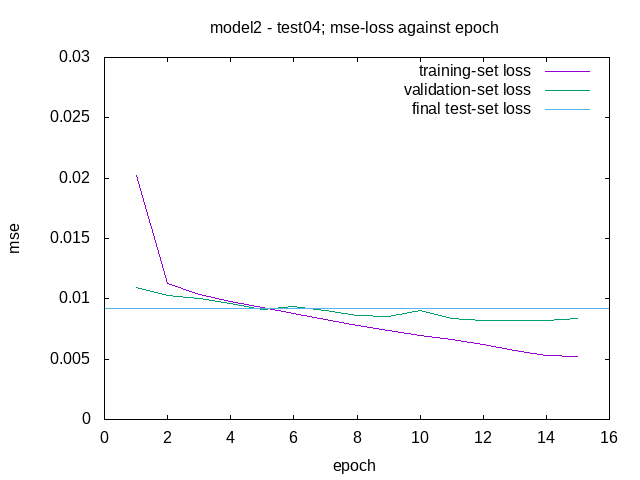
\includegraphics[scale=0.35]{model2_test04.png} & 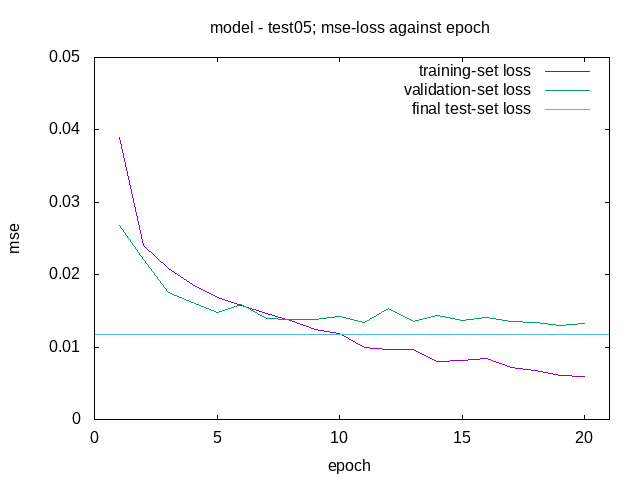
\includegraphics[scale=0.35]{./model_test05.png} \\
  \hline
\end{tabular}

\end{document}
